\chapter{Microprocessor power supply}
We want to power an STM32H4 microprocessor using a battery. The specifications are as follows:

\begin{itemize}
\item LiPo 2S battery $V_{in} = 7.4\ V$
\item Microprocessor supply voltage: $V_{out}=3.3\ V$
\item Maximum voltage ripple at the microprocessor input: $\Delta V_S = 50\ mV$
\item Output nominal current: $I_S = 200\ mA$
\item Current ripple: 30\%
\end{itemize}

To achieve this, we want to use the following component: \textbf{LT1959}, an excerpt of the documentation is attached. In this exercise, we assume that the \underline{\textbf{components are ideal}}, and that the Buck operates in \underline{\textbf{continuous conduction}} mode.

\begin{enumerate}

\item \textbf{Buck Study}

\begin{enumerate}

\item Draw the circuit to use this component in Buck operation (the values of the passive components are not required). For pin 6 $\overline{SHDN}$, assume that the Buck is always operational.

\item We assume that the processor draws a constant current $I_s$ equal to the nominal current and that the output voltage is constant (we neglect the output voltage ripple). Plot the waveform of the voltage $V_{SW}$ at the output of the \textbf{LT1959} component, the output current $I_{SW}$, the voltage $V_{ce}$ across the transistor $Q_1$, and the current $I_{L}$ through the output inductor. Deduce the relationship between the input voltage $V_{in}$, $V_{out}$, and the duty cycle $\alpha$ of the converter.

\item If the output voltage is well regulated, what will be the value of the duty cycle $\alpha_n$ imposed by the \textbf{LT1959}?

\item Justify that this component is suitable for the specifications. Can we use a LiPo 1S battery ($3.7 V$) instead of the LiPo 2S?

\item Based on the documentation, what is the switching frequency of the converter?

\item Calculate the current ripple $\Delta I_{L}$ through the output inductor, as a function of the inductance $L_1$ used. Deduce the value of the inductance to meet the specifications.

\item Plot the output voltage taking into account the voltage ripple. Calculate the value of the output capacitor $C_1$ to choose in order to meet the specifications.

\item What happens if the microprocessor consumes very little current (e.g., sleep mode)?

\end{enumerate}

\item \textbf{Control Study}

In this part, we are interested in the control of the Buck converter. For this purpose, we use the following simplified schematic:

\begin{figure}[h]
\centering
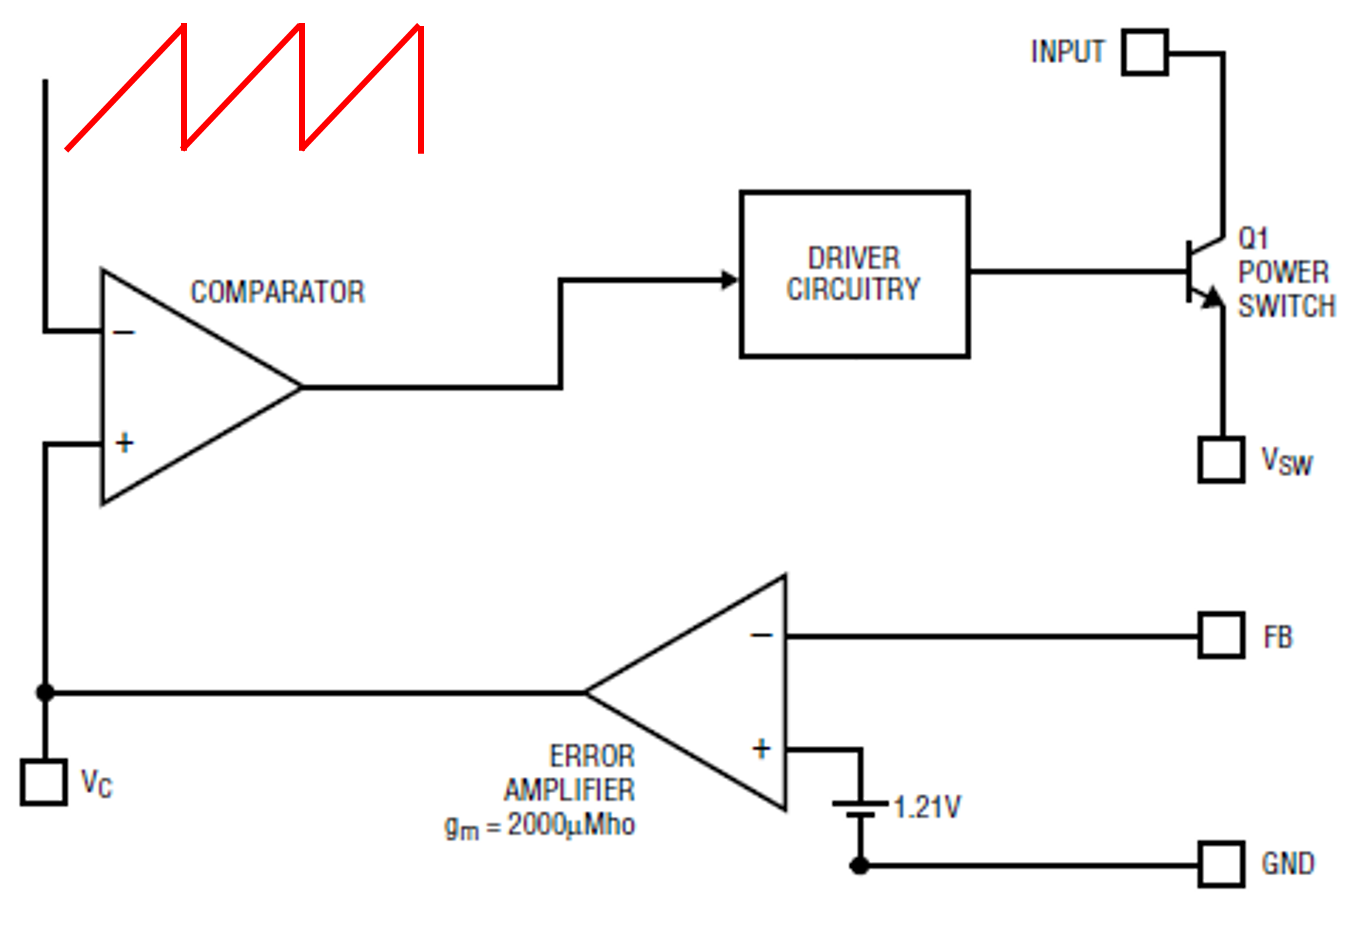
\includegraphics[width=0.8\linewidth]{TD_Buck/fig/Buck_regul.png}
\caption{Simplified internal control}
\end{figure}

The sawtooth signal varies between 0 and 2 V, with a frequency equal to the switching frequency of the converter.

\begin{enumerate}

\item Choose the values of the resistors to be connected to the \textit{FB} pin in order to obtain the desired output voltage. Use the resistor values from the E12 series.

(E12 series values: 100, 120, 150, 180, 220, 270, 330, 390, 470, 560, 680, 820).

\item For an input voltage $V^+=0.5 V$ at the comparator input, plot the output signal of the comparator. Deduce the expression that relates the comparator voltage $V^+$ and the duty cycle $\alpha$ of the converter.

The controlled converter is modeled with the following block diagram:

\begin{figure}[H]
\centering

\includegraphics[width=0.8\linewidth]{TD_Buck/fig/Buck_regul_1.png}
\caption{Global block diagram}
\end{figure}

\item Complete the ``\textit{Comparator}'' block. Using part 1, complete the ``\textit{Feedback}'' block.

The ``\textit{Buck}'' block is modeled by a static gain $K$ corresponding to $\dfrac{V_{s\ avg}}{\alpha}$ and a transfer function corresponding to the Buck output filter. The resistance $R_m$ represents the input impedance of the microcontroller.

\begin{figure}[h]
\centering

\includegraphics[width=0.55\linewidth]{TD_Buck/fig/Buck_filtre.png}
\caption{Equivalent schematic of the Buck}
\end{figure}

\item Recall the values of $L$ and $C$ determined in part 1. Determine the value of $R_m$ when the microcontroller draws the nominal current.

\item Determine the transfer function corresponding to the ``\textit{Buck}'' block.

\item A series $RC$ circuit is placed on the $V_c$ pin. We assume that the input current of the comparator is zero (high input impedance). Therefore, the ``\textit{Corrector}'' block is a proportional integral controller of the form $C(p) = K_p(1+\dfrac{1}{T_i.p})$. Determine the values of $K_p$ and $T_i$ in terms of $R$, $C$, and $g_m$.

\item Calculate $R$ so that the duty cycle at startup is approximately equal to $\dfrac{\alpha_n}{2}$ and $C$ to have a time constant of the controller 10 times greater than the time constant of the uncontrolled system.

\item In steady state, determine the output current of the error amplifier and the voltages across $R$, $C$, and $V_c$. Deduce the duty cycle and compare it to the result of 1.3.

\end{enumerate}

\end{enumerate}

\newpage
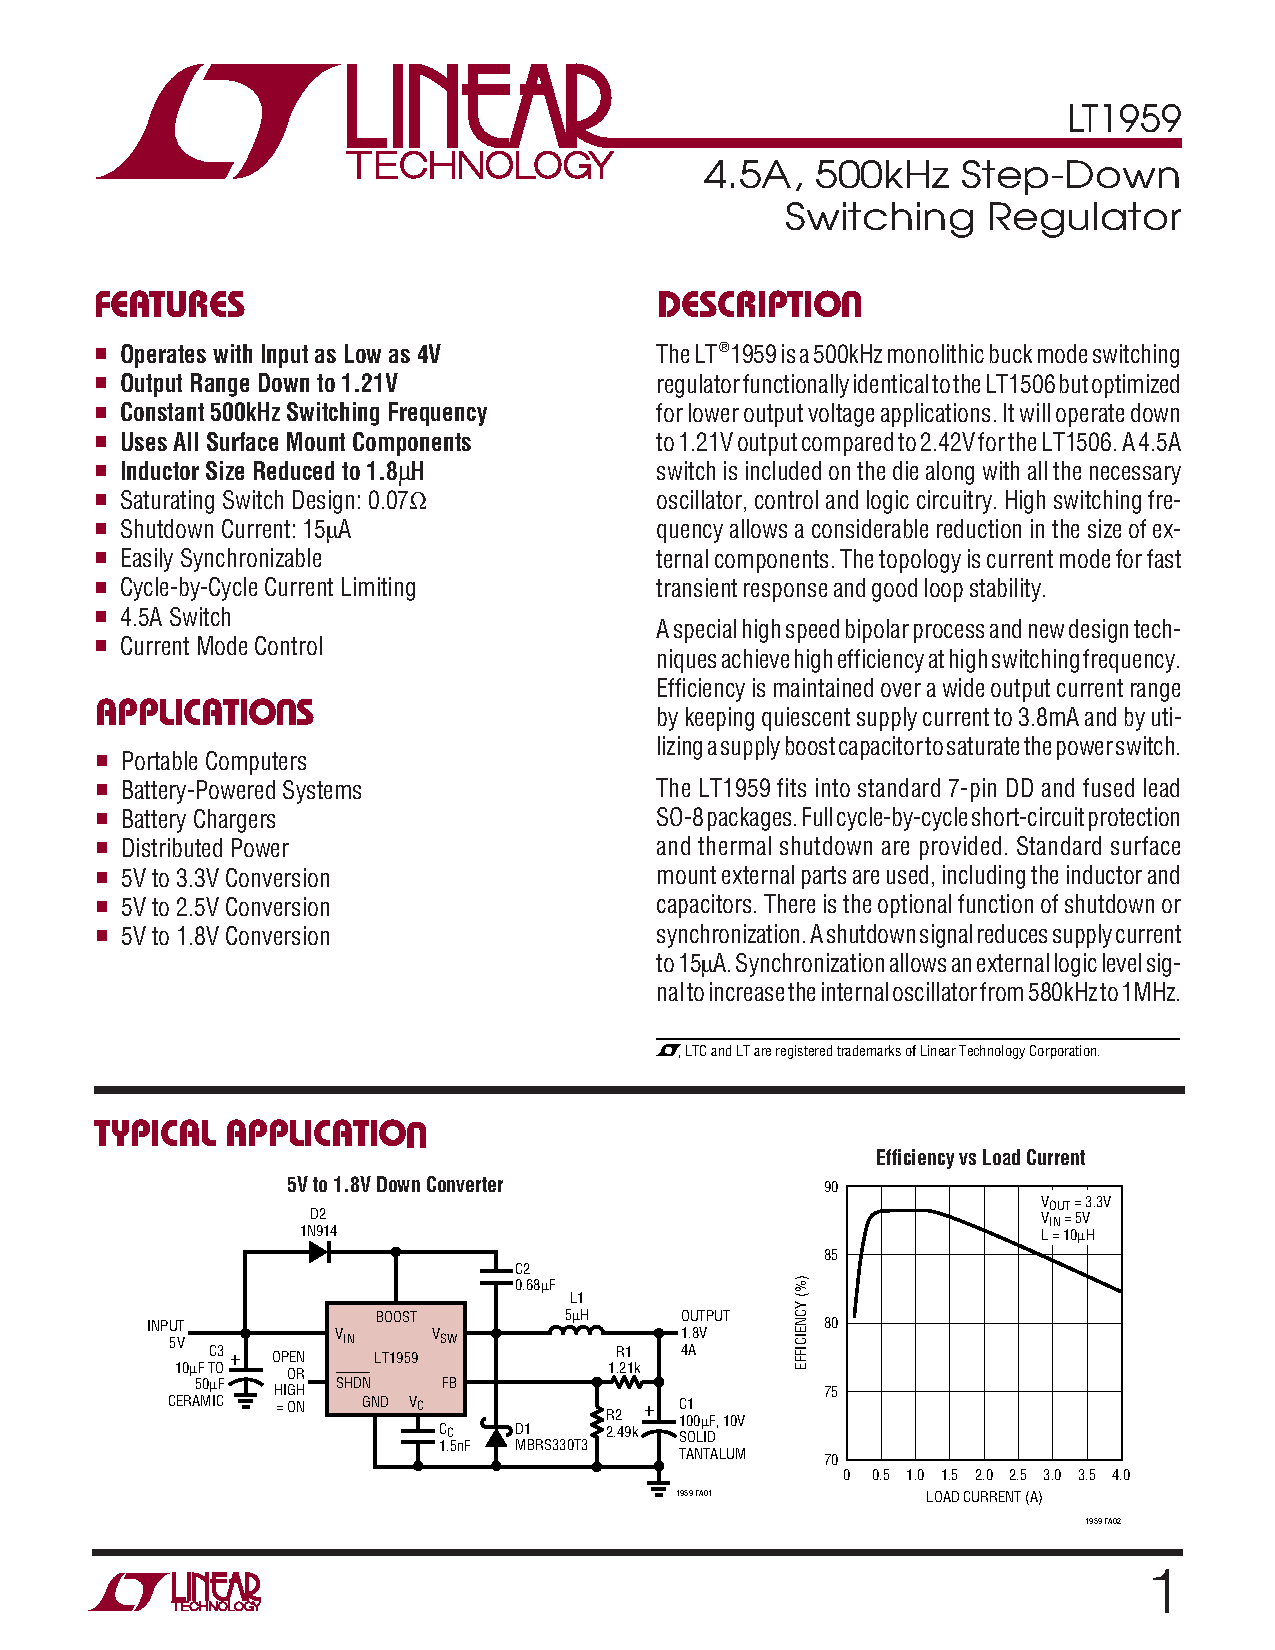
\includepdf[pages=1-4]{TD_Buck/fig/LT1959.pdf}
\includepdf[pages=6-7]{TD_Buck/fig/LT1959.pdf}
